\section{Evaluation}

\begin{frame}
        \centering
        \huge Evaluation
        \note{
                \begin{itemize}
                        \item We have evaluated specific parts and the overall system
                \end{itemize}
            }
\end{frame}

\begin{frame}
	\frametitle{Datasets}
	\begin{table}[htb]
		\centering
		\begin{tabular}{lllll}
						& Users 	& Links 		& Episodes		& Density\\
			Artificial	& \num{100}	& \num{262}		& \num{10000} 	& 2 \% \\
			Lastfm		& \num{1984}& \num{235011}	& \num{331829}	& 5 \% \\
			Weibo		& \num{5000}& \num{20784}	& \num{44345}	& 0.08 \% \\
			Twitter		& \num{4107}& \num{128855}	& \num{16824}	& 1 \%
		\end{tabular}
		\caption{Dataset Statistics}
	\end{table}
\end{frame}

\begin{frame}
	\frametitle{Baseline Approaches}
	\begin{itemize}
		\item OutDeg
		\begin{itemize}
			\item Ranks sources by their out-degree
		\end{itemize}
		\item Jordan Center
		\begin{itemize}
			\item Predicted source is the node with the minimum longest distance to any infected
		\end{itemize}
		\item Pinto's
		\begin{itemize}
			\item Assumes infection delays follows a Gaussian law
		\end{itemize}
	\end{itemize}
	\note{OutDeg: This simple baseline was used in [5]. First, we find all the “possible
		sources” i.e. all users who can reach every infected one through a series of hops in the graph. Then, we rank these possible sources by their out-degree, the higher one being the most likely source.\\
		Jordan Center: The use of a Jordan Center as a source estimator was studied	in [14]. Because our experimental context is not exactly the same as [14], we slightly adapt its formulation: the predicted source is the one with the	minimum longest distance to any infected user.\\
		Pinto’s: The model described in [16], based on the assumption that infection delays follow a Gaussian law. It uses a heuristic based on the extraction of a	tree subgraph.}
\end{frame}

\begin{frame}
	\frametitle{Training the Model}
	\begin{itemize}
		\item Value of $d = 30$
	\end{itemize}
	\begin{figure}
		\centering
		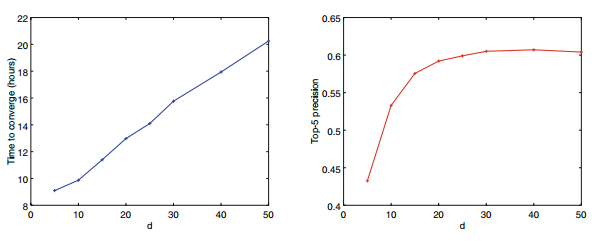
\includegraphics[scale=0.5]{convergencetime.png}
		\caption{Convergence time and performance for various values of d on the Weibo dataset}
	\end{figure}
\end{frame}